%%%%%%%%%%%%%%%%%%%%%%%%%%%%%%%%%%%%%%%%%%%%%%%%%%%%%%%%%%%%%%%%%%%%%%%%
%% Customizações do abnTeX2 (http://abnTeX2.googlecode.com)           %%
%% para a Universidade Estadual do Ceara - UECE                       %%
%%                                                                    %%
%% This work may be distributed and/or modified under the             %% 
%% conditions of the LaTeX Project Public License, either version 1.3 %%
%% of this license or (at your option) any later version.             %%
%% The latest version of this license is in                           %%
%%   http://www.latex-project.org/lppl.txt                            %%
%% and version 1.3 or later is part of all distributions of LaTeX     %%
%% version 2005/12/01 or later.                                       %%
%%                                                                    %%
%% This work has the LPPL maintenance status `maintained'.            %%
%%                                                                    %%
%% The Current Maintainer of this work is Thiago Nascimento           %%
%%                                                                    %%
%% Project available on: https://github.com/thiagodnf/uecetex2        %%
%%                                                                    %%
%% Further information about abnTeX2                                  %%
%% are available on http://abntex2.googlecode.com/                    %%
%%                                                                    %%
%%%%%%%%%%%%%%%%%%%%%%%%%%%%%%%%%%%%%%%%%%%%%%%%%%%%%%%%%%%%%%%%%%%%%%%%

%%%%%%%%%%%%%%%%%%%%%%%%%%%%%%%%%%%%%%%%%%%%%%%%%%%%%%%%%%%%%%%%%%%%%%%%
%% Customizações do abnTeX2 (http://abnTeX2.googlecode.com)           %%
%% para a Universidade Estadual do Ceara - UECE                       %%
%%                                                                    %%
%% This work may be distributed and/or modified under the             %% 
%% conditions of the LaTeX Project Public License, either version 1.3 %%
%% of this license or (at your option) any later version.             %%
%% The latest version of this license is in                           %%
%%   http://www.latex-project.org/lppl.txt                            %%
%% and version 1.3 or later is part of all distributions of LaTeX     %%
%% version 2005/12/01 or later.                                       %%
%%                                                                    %%
%% This work has the LPPL maintenance status `maintained'.            %%
%%                                                                    %%
%% The Current Maintainer of this work is Thiago Nascimento           %%
%%                                                                    %%
%% Project available on: https://github.com/thiagodnf/uecetex2        %%
%%                                                                    %%
%% Further information about abnTeX2                                  %%
%% are available on http://abntex2.googlecode.com/                    %%
%%                                                                    %%
%%%%%%%%%%%%%%%%%%%%%%%%%%%%%%%%%%%%%%%%%%%%%%%%%%%%%%%%%%%%%%%%%%%%%%%%

\documentclass[        
    a4paper,          % Tamanho da folha A4
    12pt,             % Tamanho da fonte 12pt
    chapter=TITLE,    % Todos os capitulos devem ter caixa alta
    section=TITLE,    % Todas as secoes devem ter caixa alta
    oneside,          % Usada para impressao em apenas uma face do papel
    english,          % Hifenizacoes em ingles
    spanish,          % Hifenizacoes em espanhol
    brazil            % Ultimo idioma eh o idioma padrao do documento
]{abntex2}

% Importações de pacotes

\usepackage[utf8]{inputenc}                         % Acentuação direta
\usepackage[T1]{fontenc}                            % Codificação da fonte em 8 bits
\usepackage{graphicx}                               % Inserir figuras
\usepackage{amsfonts, amssymb, amsmath}             % Fonte e símbolos matemáticos
\usepackage{booktabs}                               % Comandos para tabelas
\usepackage{verbatim}                               % Texto é interpretado como escrito no documento
\usepackage{multirow, array}                        % Múltiplas linhas e colunas em tabelas
\usepackage{indentfirst}                            % Endenta o primeiro parágrafo de cada seção.
\usepackage{listings}                               % Utilizar codigo fonte no documento
\usepackage{xcolor}
\usepackage{comment}
\usepackage{microtype}                              % Para melhorias de justificação?
\usepackage[portuguese,ruled,lined]{algorithm2e}    % Escrever algoritmos
\usepackage{algorithmic}                            % Criar Algoritmos  
%\usepackage{float}                                  % Utilizado para criação de floats
\usepackage{amsgen}
\usepackage{lipsum}                                 % Usar a simulação de texto Lorem Ipsum
%\usepackage{titlesec}                               % Permite alterar os títulos do documento
\usepackage{tocloft}                                % Permite alterar a formatação do Sumário
\usepackage{etoolbox}                               % Usado para alterar a fonte da Section no Sumário
\usepackage[nogroupskip,nonumberlist,acronym]{glossaries}                % Permite fazer o glossario
\usepackage{caption}                                % Altera o comportamento da tag caption
\usepackage[alf, abnt-emphasize=bf, bibjustif, recuo=0cm, abnt-etal-cite=3, abnt-etal-list=0,abnt-etal-text=it]{abntex2cite}  % Citações padrão ABNT
%\usepackage[bottom]{footmisc}                      % Mantém as notas de rodapé sempre na mesma posição
%\usepackage{times}                                 % Usa a fonte Times
\usepackage{mathptmx}                               % Usa a fonte Times New Roman										
%\usepackage{lmodern}                               % Usa a fonte Latin Modern
%\usepackage{subfig}                                % Posicionamento de figuras
%\usepackage{scalefnt}                              % Permite redimensionar tamanho da fonte
%\usepackage{color, colortbl}                       % Comandos de cores
%\usepackage{lscape}                                % Permite páginas em modo "paisagem"
%\usepackage{ae, aecompl}                           % Fontes de alta qualidade
%\usepackage{picinpar}                              % Dispor imagens em parágrafos
%\usepackage{latexsym}                              % Símbolos matemáticos
%\usepackage{upgreek}                               % Fonte letras gregas
\usepackage{appendix}                               % Gerar o apendice no final do documento
\usepackage{paracol}                                % Criar paragrafos sem identacao
\usepackage{lib/uecetex2}		                    % Biblioteca com as normas da UECE para trabalhos academicos
\usepackage{pdfpages}                               % Incluir pdf no documento
\usepackage{amsmath}                                % Usar equacoes matematicas

% Organiza e gera a lista de abreviaturas, simbolos e glossario
\makeglossaries

% Gera o Indice do documento
\makeindex


%%%%%%%%%%%%%%%%%%%%%%%%%%%%%%%%%%%%%%%%%%%%%%%%%%%%%
%%          Configuracoes do ueceTeX2              %%
%%%%%%%%%%%%%%%%%%%%%%%%%%%%%%%%%%%%%%%%%%%%%%%%%%%%%

% Opcoes disponiveis

%\trabalhoacademico{tccgraduacao}
%\trabalhoacademico{tccespecializacao}
\trabalhoacademico{dissertacao}
%\trabalhoacademico{tese}

% Define se o trabalho eh uma qualificacao
% Coloque 'nao' para versao final do trabalho

\ehqualificacao{nao}

% Remove as bordas vermelhas e verdes do PDF gerado
% Coloque 'sim' pare remover

\removerbordasdohyperlink{sim} 

% Adiciona a cor Azul a todos os hyperlinks

\cordohyperlink{nao}

%%%%%%%%%%%%%%%%%%%%%%%%%%%%%%%%%%%%%%%%%%%%%%%%%%%%%
%%          Informação sobre a IES                 %%
%%%%%%%%%%%%%%%%%%%%%%%%%%%%%%%%%%%%%%%%%%%%%%%%%%%%%

\ies{Universidade Estadual do Ceará}
\iessigla{UECE}
\centro{Centro de Ciências e Tecnologia}

%%%%%%%%%%%%%%%%%%%%%%%%%%%%%%%%%%%%%%%%%%%%%%%%%%%%%
%%        Informação para TCC de Graduacao         %%
%%%%%%%%%%%%%%%%%%%%%%%%%%%%%%%%%%%%%%%%%%%%%%%%%%%%%

\graduacaoem{Ciência da Computação}
\habilitacao{bacharel} % Pode colocar tambem 'licenciada'

%%%%%%%%%%%%%%%%%%%%%%%%%%%%%%%%%%%%%%%%%%%%%%%%%%%%%
%%     Informação para TCC de Especializacao       %%
%%%%%%%%%%%%%%%%%%%%%%%%%%%%%%%%%%%%%%%%%%%%%%%%%%%%%

\especializacaoem{Engenharia de Software com Ênfase em Padrões de Software}

%%%%%%%%%%%%%%%%%%%%%%%%%%%%%%%%%%%%%%%%%%%%%%%%%%%%%
%%         Informação para Dissertacao             %%
%%%%%%%%%%%%%%%%%%%%%%%%%%%%%%%%%%%%%%%%%%%%%%%%%%%%%

\programamestrado{Programa de Pós-Graduação em Ciência da Computação}
\nomedomestrado{Mestrado Acadêmico em Ciência da Computação}
\mestreem{Ciência da Computação}
\areadeconcentracaomestrado{Ciência da Computação}

%%%%%%%%%%%%%%%%%%%%%%%%%%%%%%%%%%%%%%%%%%%%%%%%%%%%%
%%               Informação para Tese              %%
%%%%%%%%%%%%%%%%%%%%%%%%%%%%%%%%%%%%%%%%%%%%%%%%%%%%%

\programadoutorado{Programa de Pós-Graduação em Ciência da Computação}
\nomedodoutorado{Doutorado em Ciência da Computação}
\doutorem{Ciência da Computação}
\areadeconcentracaodoutorado{Ciência da Computação}

%%%%%%%%%%%%%%%%%%%%%%%%%%%%%%%%%%%%%%%%%%%%%%
%%  Informação relacionadas ao trabalho     %%
%%%%%%%%%%%%%%%%%%%%%%%%%%%%%%%%%%%%%%%%%%%%%%

\autor{Nome Sobrenome}
\titulo{Título do Trabalho}
\data{2023}
\local{Fortaleza -- Ceará}

% Exemplo: \dataaprovacao{01 de Janeiro de 2012}
\dataaprovacao{}

%%%%%%%%%%%%%%%%%%%%%%%%%%%%%%%%%%%%%%%%%%%%%
%%     Informação sobre o Orientador       %%
%%%%%%%%%%%%%%%%%%%%%%%%%%%%%%%%%%%%%%%%%%%%%

\orientador{Nome do seu Orientador}
\orientadories{Universidade Estadual do Ceará – UECE}
\orientadorcentro{Centro de Ciências e Tecnologia - CCT}
\orientadorfeminino{nao} % Coloque 'sim' se for do sexo feminino

%%%%%%%%%%%%%%%%%%%%%%%%%%%%%%%%%%%%%%%%%%%%%
%%      Informação sobre o Co-orientador   %%
%%%%%%%%%%%%%%%%%%%%%%%%%%%%%%%%%%%%%%%%%%%%%

% Deixe o nome do coorientador em branco para remover do documento

\coorientador{Nome do seu Orientador}
\coorientadories{Universidade Co-orientador - SIGLA}
\coorientadorcentro{Centro do Co-orientador - SIGLA}
\coorientadorfeminino{nao} % Coloque 'sim' se for do sexo feminino

%%%%%%%%%%%%%%%%%%%%%%%%%%%%%%%%%%%%%%%%%%%%%
%%      Informação sobre a banca           %%
%%%%%%%%%%%%%%%%%%%%%%%%%%%%%%%%%%%%%%%%%%%%%

% Atenção! Deixe o nome do membro da banca para remover da folha de aprovacao

% Exemplo de uso:
% \membrodabancadois{Prof. Dr. Fulano de Tal}
% \membrodabancadoisies{Universidade Estadual do Ceará - UECE}

\membrodabancadois{Membro da Banca Dois}
\membrodabancadoiscentro{Faculdade de Filosofia Dom Aureliano Matos – FAFIDAM}
\membrodabancadoisies{Universidade do Membro da Banca Dois - SIGLA}
\membrodabancatres{Membro da Banca Três}
\membrodabancatrescentro{Centro de Ciências e Tecnologia - CCT}
\membrodabancatresies{Universidade do Membro da Banca Três - SIGLA}
\membrodabancaquatro{Membro da Banca Quatro}
\membrodabancaquatrocentro{Centro de Ciências e Tecnologia - CCT}
\membrodabancaquatroies{Universidade do Membro da Banca Quatro - SIGLA}
\membrodabancacinco{Membro da Banca Cinco}
\membrodabancacincocentro{Teste}
\membrodabancacincoies{Universidade do Membro da Banca Cinco - SIGLA}
\membrodabancaseis{Membro da Banca Seis}
\membrodabancaseiscentro{}
\membrodabancaseisies{Universidade do Membro da Banca Seis - SIGLA}

\begin{document}	

	% Se o seu trabalho é em ingles, descomente a linha a seguir
	%\selectlanguage{english}

	% Elementos pré-textuais
	\imprimircapa
	\imprimirfolhaderosto{}
	\imprimirfichacatalografica{elementos-pre-textuais/ficha-catalografica}
	\imprimirerrata{elementos-pre-textuais/errata}
	\imprimirfolhadeaprovacao
	\imprimirdedicatoria{elementos-pre-textuais/dedicatoria}
	\imprimiragradecimentos{elementos-pre-textuais/agradecimentos}
	\imprimirepigrafe{elementos-pre-textuais/epigrafe}
	\imprimirresumo{elementos-pre-textuais/resumo}
	\imprimirabstract{elementos-pre-textuais/abstract}
	\imprimirlistadeilustracoes
	\imprimirlistadetabelas
	\imprimirlistadequadros
	\imprimirlistadealgoritmos
	\imprimirlistadecodigosfonte
	\imprimirlistadeabreviaturasesiglas	
	\imprimirlistadesimbolos{elementos-pre-textuais/lista-de-simbolos}   
	\imprimirsumario
	
	%Elementos textuais
	\textual
	\chapter{Introdução}
\label{ch:introducao}

\section{Motivação}
\label{sec:motivacao}

Exemplo citação~\cite{lamport1986latex}.
%Reference without a non-breaking space 

\section{Objetivos}
\label{sec:objetivos}

\subsection{Objetivo Geral}
\label{subsec:objetivo-geral}

\subsubsection{Subsubsection}
\label{subsubsec:subsubsection}

\subsection{Objetivos Específicos}
\label{subsec:objetivos-especificos}
	\begin{alineas}
	    \item Objetivo específico 1;
		\item Objetivo específico 2;
		\item Objetivo específico 3.
	\end{alineas}

\section{E\lowercase{strutura do} T\lowercase{rabalho}}
\label{sec:estrutura-do-trabalho}
	\chapter{Fundamentação Teórica}
\label{ch:fundamentacao-teorica}

\section{F\lowercase{undamenta\c{c}\~{a}o} T\lowercase{e\'{o}rica} A}
\label{sec:fundamentacao-teorica-a}

\subsection{Subseção A.1}
\label{subsec:subsecao-a.1}

\subsection{Subseção A.2}
\label{subsec:subsecao-a.2}

\section{F\lowercase{undamenta\c{c}\~{a}o} T\lowercase{e\'{o}rica} B}
\label{sec:fundamentacao-teorica-b}

\subsection{Subseção B.1}
\label{subsec:subsecao-b.1}

\subsection{Subseção B.2}
\label{subsec:subsecao-b.2}
	\chapter{Trabalhos Relacionados}
\label{cap:trabalhos-relacionados}

\section{T\lowercase{rabalho} R\lowercase{elacionado} A}
\label{sec:trabalhos-relacionado-a}

\subsection{Subseção A.1}

\subsection{Subseção A.2}

\section{T\lowercase{rabalho} R\lowercase{elacionado} B}
\label{sec:trabalhos-relacionado-b}

\subsection{Subseção B.1}

\subsection{Subseção B.2}
	\chapter{Proposta}
\label{ch:proposta}

\lipsum[5] Conforme Figura \ref{fig:exemplo-1}.

\begin{figure}[h!]
  \centering
  \Caption{\label{fig:exemplo-1} Lorem ipsum dolor sit amet.}	
  \UECEfig{}{
  \fbox{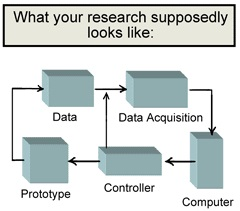
\includegraphics[width=8cm]{figuras/figura-1}}
		}{
  \Fonte{Elaborado pelo autor}
		}	
\end{figure}

\lipsum[5] Conforme Código-fonte \ref{lst-codigoCsharp}.

\begin{lstlisting}[language={[Sharp]C}, label={lst-codigoCsharp}, caption={Enumeração}]
public enum ETipoComando
{
  TIPO_0 = 0, 
  TIPO_1 = 1, // tipo 1 
  TIPO_2 = 2, // declaração do tipo 2
}
\end{lstlisting}

\lipsum[2] Conforme Algoritmo \ref{alg:algoritmo}. 

\begin{algorithm}[!ht]
  \Caption{Exemplo de Algoritmo \label{alg:algoritmo}}
  \SetSpacedAlgorithm
  \ForAll{algoritmo  $Al$}{
    Criar primeira ação do algoritmo $Al$\;
    Criar segunda ação\;
    \textbf{call} $executarComando$($Alg$)\;
    Fazer ação 1\;
    Fazer ação 2\;
    Fazer ação 3\;
    \If{possuiCondicao($Alg$)} {
      Fazer ação 4\;
    }
  }  
  \DontPrintSemicolon
  \SetKwFunction{FMain}{$executarComando$}
  \SetKwProg{Fn}{Function}{:}{}
  \Fn{\FMain{$Alg$}}{
    \ForAll{comando $Cp$ de $Alg$ }{
      Executar comando $Cp$\;  
    }
  }

\end{algorithm}

\lipsum[2] Conforme Algoritmo \ref{alg:exemplo-de-algoritmo}. 

\begin{algorithm}[!ht]  
  \Caption{\label{alg:exemplo-de-algoritmo}Como escrever algoritmos no \LaTeX2e}
  \SetSpacedAlgorithm
  \Entrada{o proprio texto}
  \Saida{como escrever algoritmos com \LaTeX2e }
  \Inicio{
    inicializa\c{c}\~ao\;
    \Repita{fim do texto}{
      leia o atual\;
      \Se{entendeu}{
        vá para o próximo\;
        próximo se torna o atual\;
        \textbf{chamar} $funcaoCom$($Parametro$)\;
      }
      \Senao{volte ao início da seção\;}
      }
  }

  \DontPrintSemicolon
  \SetKwFunction{FuncaoAuxiliar}{$funcaoCom$}
  \SetKwProg{Fn}{Funcao}{:}{}
  \Fn{\FuncaoAuxiliar{$Parametro$}}{
      \ParaTodo{elemento $p$ do $Parametro$}{
        imprimir $p$\;  
      }
    }
\end{algorithm}
	\chapter{Avaliação}
\label{ch:avaliacao}

\lipsum[5] Conforme Tabela \ref{tab:internal}.

\begin{table}[h!]	
	\centering
	\Caption{\label{tab:internal}Internal exon scores}	
	\UECEtab{}{
		\begin{tabular}{cll}
			\toprule
			Ranking & Exon Coverage & Splice Site Support\\
			\midrule \midrule
			E1 & Complete coverage by a single transcript & Both splice sites\\
			E2 & Complete coverage by more than a single transcript & Both splice sites\\
			E3 & Partial coverage & Both splice sites\\
			E4 & Partial coverage & One splice site\\
			E5 & Complete or partial coverage & No splice sites\\
			E6 & No coverage & No splice sites\\
			\bottomrule
		\end{tabular}
	}{
	\Fonte{os autores}
}
\end{table}


\lipsum[5] Conforme Tabela \ref{qua:exemplo-1}.

\begin{quadro}[h!]	
		\centering
		\Caption{\label{qua:exemplo-1} Praesent ex velit}		
		\UECEqua{}{
			\begin{tabular}{|c|c|l|l|}
				\hline
				Quisque & pharetra & tempus & vulputate \\
				\hline
				E1 & Complete coverage by a single transcript & Both  & Complete\\
				\hline
				E2 & Complete coverage by more than & Both splice sites & Complete\\
				\hline
				E3 & Partial coverage & Both splice sites & Both \\				
				\hline
			\end{tabular}
		}{
			\Fonte{Elaborado pelo autor}
		}
\end{quadro}
	\chapter{Calendário de Atividades}
\label{ch:calendario-de-atividades}



	\chapter{Conclusões e Trabalhos Futuros}
\label{ch:conclusoes-e-trabalhos-futuros}

\section{Contribuições do Trabalho}
\label{sec:contribuicoes-do-trabalho}

\section{Limitações}
\label{sec:limitacoes}

\section{Trabalhos Futuros}
\label{sec:trabalhos-futuros}





	
	%Elementos pós-textuais	
	\bibliography{elementos-pos-textuais/referencias}
	\noindent ABDULLAH, A. \textit{et al.} The duration of obesity and the risk of type 2 diabetes. \textbf{Public Health Nutrition}, Oxford, v.14, n.1, p.119-126, jan. 2011.  

\bigbreak

\noindent AEBERLI, I.; HURRELL, R.F.; ZIMMERMANN, M.B. Overweight children have higher circulating hepcidin concentrations and lower iron status but have dietary iron intakes and bioavailability comparable with normal weight children. \textbf{International Journal of Obesity}, London, v.33, n.10, p.1111– 1117, oct. 2009. 

\bigbreak

\noindent ANDRÉ, H.P. \textit{et al.} Fatores associados ao estado nutricional de ferro em crianças Brasileiras de 4 a 7 anos de idade. \textbf{Revista de Nutrição}, Campinas, v.30, n.3, p-345-355, 2017.

\bigbreak

\noindent ANDRÉ, H.P. \textit{et al.} Indicadores de insegurança alimentar e nutricional associados à anemia ferropriva em crianças brasileiras: uma revisão sistemática. \textbf{Ciência \& Saúde Coletiva}, Rio de Janeiro, v.23, n.4, p.1159-1167, abr. 2018.

\bigbreak

\noindent ANDREWS, N. C. Anemia of inflammation: the cytokine-hepcidin link. \textbf{Journal of Clinical Investigation}, New Haven, v.113, n.9, p.1251-1253, may. 2004.

\bigbreak

\noindent ANDREWS, N.C. Disorders of iron metabolism. \textbf{The New England Journal of Medicine}, Boston, v.341, n.26, p.1986–95, dec. 1999.

\bigbreak

\noindent ANDREWS, N.C. Forging a field: the golden age of iron biology. \textbf{Blood}, New York, v.112, n.2, p.219–30, jul. 2008.

\bigbreak

\noindent BAGNI, U. V.; VEIGA, G. V. Anemia ferropriva e obesidade: novos olhares para antigos problemas. Nutrire: Revista da Sociedade Brasileira de Alimentação e Nutrição. \textbf{Journal of the Brazilian Society of Food and Nutrition}, São Paulo, v. 36, n. 1, p. 177-188, abr. 2011.

\bigbreak

\noindent BAILEY, R.L. \textit{et al.} Estimation of total usual calcium and vitamin D intakes in the United States. \textbf{The Journal of Nutrition}, Rockville, v.140, n.4, p.817-822, abr. 2010.

\bigbreak

\noindent BASTARD, J.P. \textit{et al.} Recent advances in the relationship between obesity, inflammation, and insulin resistance. \textbf{European Cytokine Network}, Montrouge, v.17, n.1, p.4-12, mar. 2006.

\bigbreak

\noindent BEAUMONT, C.; VAILONT, S. Iron homeostasis. In: BEAUMONT. C.; BERIS, P.; BEUZARD, Y.; BRUGNARA, C. \textbf{Disorders of iron homeostasis, erythrocytes, erythropoiesis}. Genova, Italy: Forum Service Editore, 2006. p.393-406.

\bigbreak

\noindent BELLINASO, J. S. \textit{et al.} Educação alimentar com pré-escolares na promoção de hábitos saudáveis. \textbf{Disciplinarum Scientia}. Santa Maria, RS, v.13, n.2, p.201-215, jul. 2012.

\bigbreak

\noindent BIBBINS-DOMINGO, K. \textit{et al.} Screening for lipid disorders in children and adolescents: Us preventive services task force recommendation statement. \textbf{Journal of the American Medical Association}, Chicago, v.316, n.6, p.625-633, ago. 2016. 

\bigbreak
 
\noindent BIRCH, L. L. Development of food acceptance patterns in the first years of life. \textbf{The Proceedings of the Nutrition Society}, London, v.57, n.4, p.617-624, nov. 1998. 

\bigbreak

\noindent BIRCH, L. L.; MARLIN, D. W.; ROTTER, J. Eating as the means activity in a contingency: effects on young childrens food preferences. \textbf{Child Development}, New Jersey, v.55, n.2, p.532-539, apr. 1984.

\bigbreak

\noindent BOUGLE, D.; BROUARD, J. Iron in child obesity. Relationships with inflammation and metabolic risk factors. \textbf{Nutrients}, Basel, v.5, n.6, p.2222–30, jun. 2013.

\bigbreak

\noindent BRASIL. Ministério da Saúde. \textbf{Pesquisa Nacional de Demografia e Saúde da Criança e da Mulher – PNDS 2006: dimensões do processo reprodutivo e da saúde da criança} / Ministério da Saúde, Centro Brasileiro de Análise e Planejamento. – Brasília: Ministério da Saúde, 2009. 300 p.: il. – (Série G. Estatística e Informação em Saúde)

\bigbreak

\noindent BRASIL. Ministério da Saúde. \textbf{REDENUTRI - Evento Regional da América Latina e Caribe sobre o enfrentamento da Obesidade Infantil}. 2017. Disponível em: \url{http://ecos-redenutri.bvs.br/tiki-read\_article.php?articleId=2103}. Acesso em: 10 out 2020

\bigbreak

\noindent BRASIL. Ministério da Saúde. Secretaria de Atenção à Saúde. Departamento de Atenção Básica. \textbf{Manual das cantinas escolares saudáveis: promovendo a alimentação saudável} / Ministério da Saúde, Secretaria de Atenção à Saúde, Departamento de Atenção Básica. – Brasília: Editora do Ministério da Saúde, 2010. 56 p.: il. color. – (Série B. Textos Básicos de Saúde)

\bigbreak

\noindent BRASIL. Ministério da Saúde. Secretaria de Atenção à Saúde. Departamento de Atenção Básica. \textbf{Manual operacional para profissionais de saúde e educação: promoção da alimentação saudável nas escolas} / Ministério da Saúde, Secretaria de Atenção à Saúde, Departamento de Atenção Básica. – Brasília: Ministério da Saúde, 2008. 152 p: il. – (Série A. Normas e Manuais Técnicos)

\bigbreak

\noindent BRASIL. Ministério da Saúde. Secretaria de Atenção à Saúde. \textbf{Departamento de Atenção Básica. Saúde da criança: aleitamento materno e alimentação complementar} / Ministério da Saúde, Secretaria de Atenção à Saúde, Departamento de Atenção Básica. – 2. ed. – Brasília: Ministério da Saúde, 2015. 184 p.: il. – (Cadernos de Atenção Básica; n. 23)

\bigbreak

\noindent BRASIL. Ministério da Saúde. Secretaria de Atenção à Saúde. Departamento de Atenção Básica. \textbf{Saúde da criança: crescimento e desenvolvimento} / Ministério da Saúde, Secretaria de Atenção à Saúde, Departamento de Atenção Básica. – 1. ed. , 2. reimpressão. – Brasília: Ministério da Saúde, 2014. 272 p.: il. – (Cadernos de Atenção Básica, n. 33)

\bigbreak

\noindent BRASIL. Ministério da Saúde. Secretaria de Políticas de Saúde. Departamento de Atenção Básica. \textbf{Saúde da criança: acompanhamento do crescimento e desenvolvimento infantil} / Ministério da Saúde. Secretaria de Políticas de Saúde. - Brasília: Ministério da Saúde, 2002. 100 p.: il. - (Série Cadernos de Atenção Básica; n. 11) - (Série A. Normas e Manuais Técnicos)
\bigbreak

\noindent BROTANEK, J.M. \textit{et al.} Secular trends in the prevalence of iron deficiency among US toddlers, 1976–2002. \textbf{Archives of Pediatrics and Adolescent Medicine}, Chicago, v.162, n.4, p.374–381, apr. 2008.


\bigbreak

\noindent CARVALHO, H.B., \textit{et al.} Design and Objectives of the South American Youth/Child Cardiovascular and Environmental (SAYCARE) Study. \textbf{Obesity – A Research Journal}, v.26, suppl.1, p.5-13, 2018.

\bigbreak

\noindent CAVALCANTE, A.A.M. \textit{et al.} Consumo alimentar e estado nutricional de crianças atendidas em serviços públicos de saúde do município de Viçosa, Minas Gerais. \textbf{Revista de Nutrição}, Campinas, v.19, n.3, p.321-330, mai. Jun - 2006.

\bigbreak

\noindent COLE, T. \textit{et al.} Establishing a standard definition for child overweight and obesity worldwide: international survey. \textbf{BMJ}. v.320, p.1240-3, may, 2000; 

\bigbreak

\noindent COOK, S.; KAVEY, R.E.W. Dyslipidemia and Pediatric Obesity. \textbf{Pediatric Clinics of North America}, Philadelphia, v.58, p.58, p.1363–1373, dec. 2011.


\bigbreak

\noindent COPPACK, S. W. Pro-inflammatory cytokines and adipose tissue. \textbf{The Proceedings of the Nutrition Society}, Wallingford, v.60, n.3, p. 349-356, aug. 2001.

\bigbreak

\noindent CORRAINI, P. \textit{et al.} Effect modification, interaction and mediation: an overview of theoretical insights for clinical investigators. \textbf{Clinical Epidemiology}, v.9, p.331–8, 2017.

\bigbreak

\noindent DE FRANCA, E.; ALVES, J.G. Dislipidemia entre crianças e adolescentes de Pernambuco. \textbf{Arquivos Brasileiros de Cardiologia}, São Paulo, v.87, n.6, p.722-727, dez. 2006.

\bigbreak

\noindent DE MORAES, A.C.F. \textit{et al.} Measuring Socioeconomic Status and Environmental Factors in the SAYCARE Study in South America: Reliability of the Methods. \textbf{Obesity}, Silver Spring v.26, suppl. 1, s.14-22, mar. 2018.
\bigbreak

\noindent DGS. Direção Geral da Saúde. \textbf{Princípios para uma Alimentação Saudável}. Lisboa, 2005.

\bigbreak

\noindent INSTITUTE OF MEDICINE. \textbf{Dietary reference intakes}. 2001.

\bigbreak

\noindent EZZATI, M. \textit{et al.} Worldwide trends in body-mass index, underweight, overweight, Iand obesity from 1975 to 2016: a pooled analysis of 2416 population-based measurement studies in 128·9 million children, adolescents, and adults. \textbf{The Lancet}, London, v.390, n.10113, p.2627-2642, dec. 2017. 

\bigbreak

\noindent FAILLA, M.L.; KENNEDY, M.L.; CHEN, M.L. Iron metabolism in genetically obese (ob/ob) mice. \textbf{The Journal of Nutrition}, Rockville, v.1, n.118, p.46–51, jan. 1988. 

\bigbreak

\noindent FAIN, J.N. Release of interleukins and other inflammatory cytokines by human adipose tissue is enhanced in obesity and primarily due to the nonfat cells. \textbf{Vitamins and Hormones}, New York, v.74, p.443-477, 2006.

\bigbreak

\noindent FAIRBANKS, V.G.; BEUTLER, E. Iron metabolism. In: BEUTLER, E.; LICHTMAN, M.A.; COLLER, B.S.; KIPPS, T.J.; SELIGSOHN, U. \textbf{Williams-Hematology}, 6th. ed. New York: Mcgraw-Hill; 2001, p. 295-304.  

\bigbreak

\noindent FERNANDES, F. M. \textbf{Alimentação e nutrição entre escolares: caso dos alunos de uma escola do município, Vitória – ES}. 2006. 49 f. Monografia (Especialização em Nutrição Clínica) - Curso de Pós-Graduação em Nutrição Clínica, Universidade Veiga de Almeida, Vitória, 2006.

\bigbreak

\noindent FERNÁNDEZ-ALVIRA, J.M. \textit{et al.} Parental education associations with children’s body composition: mediation effects of energy balance-related behaviors within the ENERGY-project. \textbf{International Journal of Behavioral Nutrition and Physical Activity}, p.10-80, jun. 2013. 

\bigbreak

\noindent FILHA, E. O. S. \textit{et al.} Consumo dos grupos alimentares em crianças usuárias da rede pública de saúde do município de Aracaju, Sergipe. \textbf{Revista Paulista de Pediatria}, São Paulo, v.30, n.4, p.529-536, jun. 2012.

\bigbreak

\noindent FLEMING, R. E. Iron and inflammation: cross-talk between pathways regulating hepcidin. \textbf{Journal of Molecular Medicine}, Berlin, v.86, n.5, p.491-494, may, 2008.

\bigbreak

\noindent FOX, M. K. \textit{et al.} Relationship between portion size and energy intake among infants and toddlers: evidence of self-regulation. \textbf{Journal of the American Dietetic Association}, Chigaco, v.106, suppl.1, s.77-83, 2006.

\bigbreak

\noindent FREEDMAN, D.S. \textit{et al.} Cardiovascular risk factors and excess adiposity among overweight children and adolescents: the Bogalusa Heart Study. \textbf{The Journal of Pediatrics}, Saint Louis, v.150, n.1, p.12-17, jan. 2007.

\bigbreak

\noindent FROTA, M.A.; BARROSO, M.G.T. Repercussão da desnutrição infantil na família. \textbf{Revista Latino-americana de Enfermagem}, Ribeirão Preto, v.13, n.6, p.996-1000, nov. – dez. 2005.

\bigbreak

\noindent GAGLIONE, C. P. Alimentação no segundo ano de vida, pré-escolar e escolar. In: LOPES, F. A.; BRASIL, A. L. D. \textbf{Nutrição e Dietética em Clínica Pediatria}. São Paulo: Atheneu, 2003. p.61-62 

\bigbreak

\noindent GANZ, T.; NEMETH, E. Iron imports. IV. Hepcidin and regulation of body iron metabolism. \textbf{American Journal of Physiology - Gastrointestinal and Liver Physiology}, Bethesda, v.290, n.2, p.199-203, feb. 2006.

\bigbreak

\noindent GARROW, J.S. \textbf{Obesity and related diseases}. London, Churchill Livingstone, p.1-16, 1988. 

\bigbreak

\noindent GIULIANO, I.C.B. \textit{et al.} Lípides séricos em crianças e adolescentes de Florianópolis, SC – Estudo Floripa saudável 2040. \textbf{Arquivos Brasileiros de Cardiologia}, São Paulo, v.85, n.2, p.85-91, ago. 2005.

\bigbreak

\noindent GOMES, E.; ZAGO, V.H.S.; FARIA, E.C. Avaliação de Perfis Lipídicos Infanto-Juvenis Solicitados nas Unidades Básicas de Saúde em Campinas/SP, Brasil: Um Estudo Laboratorial Transversal. \textbf{Arquivos Brasileiros de Cardiologia}, São Paulo, v.114, n.1, p.47-56, jan. 2020.

\bigbreak

\noindent GRAF, L. \textit{et al.} Old and new iron parameters in iron metabolism and diagnostics. \textbf{Therapeutische Umschau. Revue therapeutique}, Bern, v.65, n.9, p.519-28, sep. 2008.

\bigbreak

\noindent GRAHAM JR. \textit{et al.} Policy Statement. Organizational principles to guide and define the child health care system and/or improve the health of all children. \textbf{American Academy Of Pediatrics}, v.116, n.6, p.1574-1575, 2005. 

\bigbreak

\noindent GROTTO, H.Z.W. Diagnóstico laboratorial da deficiência de ferro. \textbf{Revista Brasileira de Hematologia e Hemoterapia}, São Paulo, v.32, supl.2, p22-28, jun. 2010.

\bigbreak

\noindent GROTTO, H. Z.W. Metabolismo Do Ferro: Uma revisão sobre os principais mecanismos envolvidos em sua homeostase. \textbf{Revista Brasileira de Hematologia e Hemoterapia}, São Paulo, v.30, n.5, p. 390-397, 2008.

\bigbreak

\noindent GUTHRIE, H. A. \textit{et al.} Hyperlipidemia in offspring of iron deficient rats. \textbf{The Journal of Nutrition}, Rockville, v.104, n.10, p.1273–1278, oct. 1974.

\bigbreak

\noindent HENRIQUES, G.S.; DE ALENCAR, L.L.; COZZOLINO, S.M.F. Ferro. In: COZZOLINO, S.M.F. [Org.]. \textbf{Biodisponibilidade de nutrientes}. 5.ed. rev. e atual. Barueri, SP: Manole, 2016. cap.27, p.673-704

\bigbreak

\noindent HERRINGTON, L. \textit{et al.} Factors affecting pediatric dyslipidemia screening and treatment. \textbf{Clinical Pediatrics}, Thousand Oaks, v.58, n.5, p.502-510, may. 2019.

\bigbreak

\noindent HOFFBRAND, A.V.; PETTIT, F.E.; MOSS, P.A.H. \textbf{Hypochromic anaemias and iron overload}. 5thed. Oxford (UK): Blackwell Publishing, 2006, cap.3, p. 28-43. 

\bigbreak

\noindent HUXLEY, R. \textit{et al.} Body Mass Index, waist circumference and waist: Hip ratio as predictors of cardiovascular risk - a review of the literature. \textbf{European Journal of Clinical Nutrition}, London, v.64, n.1, p.16-22, jan. 2010.

\bigbreak

\noindent INGE, T.H. \textit{et al.} The effect of obesity in adolescence on adult health status. \textbf{Pediatrics}, Elk Grove, v.132, n.6, p.1098-1104, dec. 2013. 

\bigbreak

\noindent IRALA, C. H.; FERNANDEZ, P. M. Peso Saudável. Manual para Escolas. A Escola promovendo hábitos alimentares saudáveis. Faculdade de Ciências da Saúde, \textbf{Departamento de Nutrição}. Universidade de Brasília, 2001. Disponível em: \url{http://189.28.128.100/nutricao/docs/geral/pesoSaudavel.pdf}. Acesso em: 05 set 2020. 

\bigbreak

\noindent JUONALA, M. \textit{et al.} Childhood adiposity, adult adiposity, and cardiovascular risk factors. \textbf{New England Journal of Medicine}, Massachusetts, v.365, n.20, p.1876-1885, nov. 2011.

\bigbreak

\noindent JUONALA, M. \textit{et al.} Main findings from the prospective Cardiovascular Risk in Young Finns Study. \textbf{Current Opinion in Lipidogy}, England, v.24, n.1, p.57-64, fev. 2013.

\bigbreak

\noindent KRANZ, S. \textit{et al.} What do we know about dietary fiber intake in children and health? The effects of fiber intake on constipation, obesity, and diabetes in children. \textbf{Advances in Nutrition}, Bethesda, v.3, n.1, p.47-53, jan. 2012.

\bigbreak

\noindent KRAUSE, A. \textit{et al.} LEAP-1, a novel highly disulfide-bonded human peptide, exhibits antimicrobial activity. \textbf{FEBS Letters}, Amsterdã (Publisher) ou West Sussex, v.480, n. 2-3, p. 147-150, sep. 2000.
\bigbreak

\noindent KRAUSE, R. F. Changes induced by anemia in the bone marrow lipids of cats. \textbf{Journal of Biological Chemistry}, New York, v.149, p.395-404, may. 1943.

\bigbreak

\noindent LACERDA, E.M.A.; ACCIOLLY, E. Alimentação do Pré-Escolar e Escolar. In: ACCIOLLY, E.; SAUNDERS, C.; LACERDA, E.M.A. \textbf{Nutrição em Obstetrícia e Pediatria}. 3ª reimpressão. Rio de Janeiro: Cultura Médica, 2005. Cap.19, p.369-382. 

\bigbreak

\noindent LEAL, K.K. \textit{et al.} Qualidade da dieta de pré-escolares de 2 a 5 anos residentes na área urbana da cidade de Pelotas, RS. \textbf{Revista Paulista de Pediatria}, São Paulo, v.33, n.3, p.310-317, jun. 2015.

\bigbreak

\noindent LEONG, W.; LÖNNERDAL, B. Hepcidin, the recently identifi ed peptide that appears to regulate iron absorption. The Journal of Nutrition, Rockville, v.134, n.1, p.1-4, jan. 2004.

\bigbreak

\noindent LI, B. \textit{et al.} Study of the correlation between serum ferritin levels and the aggregation of metabolic disorders in non-diabetic elderly patients. \textbf{Experimental and Therapeutic Medicine}, Athens, v.7, n.6, p.1671-1676, jun. 2014.

\bigbreak

\noindent LIKERT, R. A technique for the measurement of attitudes. \textbf{Archives of Psychology}, v.22, n.140, p.55, 1982. 

\bigbreak

\noindent LIMA, Gabriela Guirao Bijos. \textbf{O educador promovendo hábitos alimentares saudáveis por meio da escola}. 2008. Disponível em: \url{https://pt.scribd.com/document/159601032/Gabriela-Lima}. Acesso em: 10 out 2020

\bigbreak

\noindent MACKINNON, D. \textbf{Introduction to statistical mediation analysis}. New York: Erlbaum, 2008.

\bigbreak

\noindent MAGALHÃES, \textit{et al.} Fatores associados à dislipidemia em crianças de 4 a 7 anos de idade. \textbf{Revista de Nutrição}, Campinas, v.28, n.1, jan. - fev. 2015.

\bigbreak

\noindent MASON, B.H.; MOORE, C. B. \textbf{Principles of Geochemistry}. 4thed. Wiley: New York, 1982, 344p 

\bigbreak

\noindent MCCLUNG, J. P.; KARL, J. P. Iron deficiency and obesity: the contribution of inflammation and diminished iron absorption. \textbf{Nutrition Reviews}, Washington, v.67, n.2, p.100-104, feb. 2009.

\bigbreak

\noindent MENA, N. P. \textit{et al.} Hepcidin inhibits apical iron uptake in intestinal cells. \textbf{American Journal of Physiology. Gastrointestinal and Liver Physiology}, Bethesda, v.294, n.1, p.192-198, jan. 2008. 

\bigbreak

\noindent NAOUM, F.A. Alterações do perfil lipídico nas anemias. \textbf{Revista Brasileira de Hematologia e Hemoterapia}, São José do Rio Preto, v.27, n.3, p.223-226, jul. - set. 2005.

\bigbreak

\noindent NASCIMENTO, B.R. \textit{et al.} Epidemiologia das Doenças Cardiovasculares em Países de Língua Portuguesa: Dados do “Global Burden of Disease”. 1990 a 2016. \textbf{Arquivos Brasileiros de Cardiologia}, São Paulo, v.110, n.6, p.500-511, jun. 2018.

\bigbreak

\noindent NELSON, M. Anaemia in adolescent girls: effects on cognitive function and activity. \textbf{The Proceedings of the Nutrition Society}, London, v.55, n.1B, p.359-367, mar. 1996.

\bigbreak

\noindent NEMETH, E.; GANZ, T. Regulation of iron metabolism by hepcidin. \textbf{Annual Review of Nutrition}, Palo Alto, v.26, p.323-342, 2006.

\bigbreak

\noindent OGATA, B.; FEUCHT, S.A.; LUCAS, B.L. Nutrição na Infância. In: L. Kathleen Mahan, Janice L. Raymond; [tradução Verônica Mannarino, Andréa Favano]. \textbf{Krause alimentos, nutrição e dietoterapia}. 14.ed. Rio de Janeiro: Elsevier, 2018. cap. 17, p.313-329.

\bigbreak

\noindent OGDEN, J. \textbf{The Psychology of Eating From Healthy to Disordered Behaviour}. 1ed. United Kingdom: Blackwell Publishing. 2003.

\bigbreak

\noindent OPAS, Organização Pan-Americana de Saúde. \textbf{Mais de um em cada três países de baixa e média renda enfrentam extremos da má nutrição}. 2019b. Disponível em: \url{https://www.paho.org/bra/index.php?option=com\_content\&view=article\&id=6082:mais-de-um-em-cada-tres-paises-de-baixa-e-media-renda-enfrentam-extremos-da-ma-nutricao\&Itemid=839}. Acesso em: 20 de out 2020

\bigbreak

\noindent OPAS. Organização Pan-Americana de Saúde. \textbf{Folha informativa – Alimentação saudável}. 2019a. Disponível em: \url{https://www.paho.org/bra/index.php?option=com\_content\&view=article\&id=5964:folha-informativa-alimentacao-saudavel\&Itemid=839}. Acesso em: 10 de set 2020

\bigbreak

\noindent PARK, C. H. \textit{et al.} Hepcidin, a urinary antimicrobial peptide synthesized in the liver. \textbf{Journal of Biological Chemistry}, Baltimore, v.276, n.11, p.7806-910, mar. 2001.

\bigbreak

\noindent PERGHER, R.N.Q. \textit{et al.} O diagnóstico de síndrome metabólica é aplicável às crianças? \textbf{Jornal de Pediatria}, Rio de Janeiro, v.86, n.2, p101-108, 2010.

\bigbreak

\noindent PETERSON, A.L. \textit{et al.} JCL roundtable: Pediatric lipidology. \textbf{Journal of Clinical Lipidology}, New York, v.13, n.5, p.676-688, oct. 2019.
 
\bigbreak

\noindent PHILIPPI, Sonia Tucunduva. \textbf{Tabela de composição de alimentos para suporte nutricional}. 2ed. São Paulo: Coronário, 2002.

\bigbreak

\noindent PHILIPPI, S.T. \textit{et al.} Pirâmide alimentar para crianças de 2 a 3 anos. \textbf{Revista de Nutrição}, Campinas, v.16, n.1, p.5-19, jan. - mar. 2003.

\bigbreak

\noindent PINHAS-HAMIEL, O. \textit{et al.} Greater prevalence of iron deficiency in overweight and obese children and adolescents. \textbf{International Journal of Obesity and Related Metabolic Disorders}, Hampshire, v.27, n.3, p.416–418, mar. 2003.

\bigbreak

\noindent PINHEIRO, D. S. \textit{et al.} Intervenção escolar na educação alimentar infantil quanto aos micronutrientes. \textbf{Revista da Universidade Vale do Rio Verde}, Três Corações, v.10, n.1, p.209-217, 2012.

\bigbreak

\noindent POPKIN, B. M. The nutrition transition in low‐income countries: an emerging crisis. \textbf{Nutrition reviews}, Washington, v.52, n.9, p.285-298. sep. 1994. 

\bigbreak

\noindent PORTO, E.B.S. \textit{et al.} As cantinas escolares do Distrito Federal, Brasil e a promoção da alimentação saudável. \textbf{Revista de Nutrição}, Campinas. v.28, n.1, p.29-41, jan. - fev.; 2015.

\bigbreak

\noindent RIVERA, J.A. \textit{et al.} Introduction to the double burden of undernutrition and excess weight in Latin America. \textbf{The American journal of clinical nutrition}, Rockville, v.100, n.6, S1613-1616, dec. 2014.

\bigbreak

\noindent SAPUNAR, J. \textit{et al.} A. High prevalence of dyslipidemia and high atherogenic index of plasma in children and adolescents. \textbf{Revista Médica de Chile}, Santiago, v.146, n.10, p.1112-1122, dec. 2018.

\bigbreak

\noindent SARAVIA, L. \textit{et al.} Development of a Food Frequency Questionnaire for Assessing Dietary Intake in Children and Adolescents in South America. \textbf{Obesity}, Silver Spring, v.26, suppl. 1, mar. 2018.

\bigbreak

\noindent SBC, Sociedade Brasileira de Cardiologia.  \textbf{Atualização da Diretriz Brasileira de Dislipidemias e Prevenção da Aterosclerose}, v.109. n.1, 2017.

\bigbreak

\noindent SBP. Sociedade Brasileira de Pediatria. Departamento de Nutrologia. \textbf{Manual de Alimentação: orientações para alimentação do lactente ao adolescente, na escola, na gestante, na prevenção de doenças e segurança alimentar}. 4ed. São Paulo: SBP, 2018. 172p

\bigbreak

\noindent SBP. Sociedade Brasileira de Pediatria. Guia Prático de Atualização. Departamento Científico de Endocrinologia (2019-2021). \textbf{Dislipidemia na criança e no adolescente - Orientações para o pediatra}. n.8, mai. 2020, 13p

\bigbreak

\noindent SBP, Sociedade Brasileira de Pediatria. \textbf{Novas orientações sobre o jejum para a determinação laboratorial do perfil lipídico}. Guia Prático de Atualização. Departamento Científico de Endocrinologia, Sociedade Brasileira de Pediatria. jun. 2017.

\bigbreak

\noindent SCHOENBUCHNER, S.M. \textit{et al.} The relationship between wasting and stunting: a retrospective cohort analysis of longitudinal data in Gambian children from 1976–2016. \textbf{American Journal of Clinical Nutrition}, v.110, n.2, p.498–507, 2019.

\bigbreak

\noindent SELA, B. A. Hepcidin-the discovery of a small protein with a pivotal role in iron homeostasis. \textbf{Harefuah}, Tel Aviv, v.147, n.3, p.261-276, mar. 2008.

\bigbreak

\noindent SELTZER CC, MAYER J. Serum iron and iron-binding capacity in adolescents. II. Comparison of obese and nonobese subjects. \textbf{The American Journal of Clinical Nutrition}, Bethesda, v.13, p.354–361, dec. 1963. 

\bigbreak

\noindent SENGSUK, C. \textit{et al.} Association of Iron Overload with oxidative stress, Hepatic Damage and Dyslipidemia in Transfusion-Dependent beta-Thalassemia/HbE Patients. \textbf{Indian Journal of Clinical Biochemistry}, New Delhi, v.29, n.3, p.298-305, jul. 2014.

\bigbreak

\noindent SHERMAN, A. R. Serum lipids in suckling and postweaning iron deficient rats \textbf{Lipids}, Chicago, v.14, n.11, p.888-892, nov. 1979.

\bigbreak

\noindent SHRIMPTON, R.; ROKX, C. The double burden of malnutrition: A review of global evidence. In: \textbf{NETWORK, Human Development (ed.)}. The World Bank’s: Washington, 2012.

\bigbreak

\noindent SPARRENBERGER, K. \textit{et al.} Consumo de alimentos ultraprocessados entre crianças de uma Unidade Básica de Saúde. \textbf{Jornal de Pediatria}. (Rio J.) [online], Porto Alegre, v.91, n.6, p.535-542, nov. - dez. 2015.

\bigbreak

\noindent STOPLER, Tracy; WEINER, Susan. Terapia de Nutrição Médica para Anemia. In: MAHAN, L. K.; RAYMOND, J.L. [tradução Verônica Mannarino, Andréa Favano]. \textbf{Krause alimentos, nutrição e dietoterapia}. 14. ed. Rio de Janeiro: Elsevier, 2018 cap. 32, p.630-645.

\bigbreak

\noindent SULLIVAN, J.L. Iron and the sex difference in heart disease risk. \textbf{Lancet}, London, v.1, n.8233, p.1293-1294, jun.1981.

\bigbreak

\noindent SULLIVAN, J.L. Iron in arterial plaque: modifiable risk factor for atherosclerosis. \textbf{Biochimica et Biophysica Acta}, Amsterdam, v.1790, n.7, p.718-723, jul. 2009.

\bigbreak

\noindent SULLIVAN, S. A.; BIRCH, L. L. Infant dietary experience and acceptance of solid foods. \textbf{Pediatrics}, Springfield, v.93, n.2, p.271-277, feb. 1994. 

\bigbreak

\noindent TANZER, F. \textit{et al.} Serum free carnitine and total triglycerid levels in children with iron deficiency anemia. \textbf{International journal for vitamin and nutrition research}, Bern, v.71, n.1, p.66–69, jan. 2001.

\bigbreak

\noindent TEMPONI, H. R.; VELASQUEZ-MELENDEZ, G. Prevalência de dupla carga de má nutrição em nível domiciliar em quatro países da América Latina. \textbf{Revista Brasileira de Saúde Materno Infantil}, Recife, v.20, n.1, p.37-45, jan. - mar. 2020.

\bigbreak

\noindent TEODORO, M.A. \textit{et al.} Estratégia de educação alimentar e nutricional na prevenção de distúrbios nutricionais em pré-escolares. \textbf{Revista Eletrônica de Extensão}, Florianópolis, v.15, n.31, p.15-30, 2018.

\bigbreak

\noindent \textbf{THE LANCET}, A future direction for tackling malnutrition. \textbf{The Lanccet}, London, v. 395, n. 10217, p. 2, 2020. Editorial. Disponível em: \url{https://www.thelancet.com/action/showPdf?pii=S0140-6736\%2819\%2933099-5}. Acesso em: 10 out 2020

\bigbreak

\noindent TUSSING-HUMPHREYS, L.M. \textit{et al.} Excess adiposity, inflammation, and iron deficiency in female adolescents. \textbf{Journal of the American Dietetic Association}, Chicago, v.109, n.2, p.297–302, feb. 2009. 

\bigbreak

\noindent TZIOUMIS, E.; ADAIR, L. S. Childhood dual burden of under-and overnutrition in low-and middle-income countries: a critical review. \textbf{Food and Nutrition Bulletin}, Tokyo, v.35, n.2, p.230-243. Jun. 2014.

\bigbreak

\noindent VIANA, V.; SANTOS, P.L.; GUIMARÃES, M.J. Comportamento e hábitos alimentares em crianças e jovens: uma revisão da literatura. \textbf{Psicologia, Saúde e Doenças}. Lisboa, v.9, n.2, p.209-31, jun. – set. 2008.

\bigbreak

\noindent VIEIRA, R.C.S.; FERREIRA, H.S. Prevalência de anemia em crianças brasileiras, segundo diferentes cenários epidemiológicos. \textbf{Revista de Nutrição}, Campinas, v.23, n.3, p.433-444, mai. –jun. 2010.

\bigbreak

\noindent VITOLO, Márcia Regina. \textbf{Nutrição da gestação ao envelhecimento}. Rio de Janeiro: Rubio, 2015.

\bigbreak

\noindent VITOLO, Márcia Regina. Recomendações nutricionais para crianças. In: \_\_\_\_\_\_. \textbf{Nutrição da gestação ao envelhecimento}. Rio de Janeiro: Rubio, 2008: 191-9.

\bigbreak

\noindent WATERLOW J. C. Classification and definition of protein-calorie Malnutrition. \textbf{British medical journal}, v.3, n.5826, p.566-569, sep. 1972.

\bigbreak

\noindent WHO. World Health Organization. \textbf{Complementary feeding of young children in developing countries: a review of current scientific knowledge}. Geneva: WHO, 1998.

\bigbreak

\noindent WHO. World Health Organization. \textbf{Development of a WHO growth reference for school-aged children and adolescents}. Bulletin of the World Health Organization. v.85, p.660-667, 2007. 

\bigbreak

\noindent WHO. World Health Organization. \textbf{Exclusive breastfeeding for six months best for babies everywhere}. 2011. Disponível em: \url{https://www.who.int/news/item/15-01-2011-exclusive-breastfeeding-for-six-months-best-for-babies-everywhere}. Acesso em: 20 set 2020

\bigbreak

\noindent WHO. World Health Organization. \textbf{Iron deficiency anemia:} assessment, prevention and control. A guide for programme managers. Document WHO/NHD/01.3. Geneva: World Health Organization, 2001.

\bigbreak

\noindent WHO. World Health Organization. \textbf{Obesity:} preventing and managing the global epidemic. Report of a WHO Consultation. Geneva: World Health Organization; 2000. (WHO Technical Report Series, 894).

\bigbreak

\noindent WHO. World Health Organization. \textbf{Physical Status: Uses and Interpretation of Anthropometry}. WHO Technical Report Series, Report n.854. Geneva, Switzerland: WHO. 1995.

\noindent WHO. World Health Organization. \textbf{World Obesity Day}. 2020. Disponível em: \url{https://www.who.int/news-room/events/detail/2020/03/04/default-calendar/world-obesity-day}. Acesso em: 15 de out 2020

\bigbreak

\noindent WIJAYANTI, N.; KATZ, N.; IMMENSCHUH, S. Biology of heme in health and disease. \textbf{Current Medicinal Chemistry}, Schiphol, v.11, n.8, p.981-986, apr. 2004.

\bigbreak

\noindent YANOFF, L.B. \textit{et al.} Inflammation and iron deficiency in the hypoferremia of obesity. \textbf{International Journal of Obesity}, London, v.31, n.9, p.1412–1419, set. 2007. 

\bigbreak

\noindent ZACHARIAH, J.P.; JOHNSON, P.K. Pediatric lipid management. \textbf{Endocrinology and Metabolism Clinics of North America}, v.43, n.4, p.981- 992, dec. 2014.

\bigbreak

\noindent ZHAO, L. \textit{et al.} Obesity and iron deficiency: a quantitative meta-analysis. \textbf{Obesity Reviews}, v.16, n.12, p.1081–1093, dec. Oxford, 2015. 

\bigbreak

\noindent ZHU, Y. \textit{et al.} Iron metabolism and its association with dyslipidemia risk in children and adolescents: a cross-sectional study. \textbf{Lipids in Health and Disease}, London, v.18, n.50, p.1-8, feb. 2019.

\bigbreak

\noindent ZIMMERMANN, M. B. \textit{et al.} Adiposity in women and children from transition countries predicts decreased iron absorption, iron deficiency and a reduced response to iron fortification. \textbf{International Journal of Obesity}, London, v.32, n.7, p.1098-1104, jul. 2008.

	
	\imprimirglossario	
	\imprimirapendices
		% Adicione aqui os apendices do seu trabalho
		\apendice{Título Apêndice A}
\label{ap:titulo-apendice-a}

\section{S\lowercase{e\c{c}\~ao} A}
\label{sec:secao-a}

\subsection{Subseção A.1}
\label{subsec:subsecao-a.12}

\subsection{Subseção A.2}
\label{subsec:subsecao-a.22}

\section{S\lowercase{e\c{c}\~ao} B}
\label{sec:secao-b}

\subsection{Subseção B.1}
\label{subsec:subsecao-b.12}

\subsection{Subseção B.2}
\label{subsec:subsecao-b.22}
	\imprimiranexos
		% Adicione aqui os anexos do seu trabalho
		\anexo{Exemplo de Anexo}
\label{an:exemplo-de-anexo}

\lipsum[13]		
		\anexo{Dinâmica das classes sociais}
\label{an:dinamica-das-classes-sociais}

\lipsum[14]
\index{AAA}
	\imprimirindice

\end{document}